%%%%%%%%%%%%Outline%%%%%%%%%%%%%%%%%%

%%% Section 4 \lang Design

%%%
% message<opening: each \lang opcode carries two representations, proof sequence for verification and native emit for execution>
% each \lang opcode carries two representations: proof sequence + native emit callback
% proof sequence: short fragment of vanilla eBPF defining the opcode's semantics
% native emit: produces hardware-specific machine code inserted into the JIT image
% \lang opcodes have their own encoding, verifier path, and JIT dispatch
% §4.1 principles and challenges, §4.2 pipeline

%%% Section 4.1 Design Principles and Challenges

%%%
% message<performance gap (§3) and formal verification constraints (§2.3) motivate four design principles>
% verifier's core analysis (abstract interpretation, transfer functions) must not change
% cross-instruction pattern recognition in compiler at compile time, not in JIT at translation time
% extensible: new instruction = new module, no kernel core changes
% backward compatible: programs without \lang compile and execute identically to unmodified eBPF

%%%
% message<three concrete challenges>
% meta-sentence: these principles lead to three concrete challenges

%%%
% message<C1: verification without new transfer functions>
% verifier defines one transfer function per opcode, rejects unknown opcodes
% new opcode ordinarily requires new transfer function with type rules and range tracking
% \lang must let verifier accept new opcodes without adding transfer functions

%%%
% message<C2: JIT translation without hardcoded opcodes>
% JIT has fixed switch over known opcodes, per-architecture
% new opcode requires new case in every backend, must be known at compile time
% \lang must let JIT emit native code for externally-defined opcodes

%%%
% message<C3: arch-specific execution with arch-independent verification>
% different platforms have different native instructions (ROL vs ROR)
% execution must be platform-specific; verification must be architecture-independent
% \lang must separate these without duplicating the safety argument per architecture

%%% Section 4.2 Compilation Pipeline with \lang

%%%
% message<overview: compilation → verification (lower/verify/restore) → execution (native emit)>
% LLVM backend compiles C to \lang bytecode, encoding multi-instruction patterns as extended opcodes
% kernel verifier lowers extended opcodes to proof sequences, verifies, restores
% JIT dispatches each extended opcode to module-provided native emit callback
% each mechanism addresses one challenge from §4.1; figure shows end-to-end pipeline

%%%
% message<lowering \lang to vanilla eBPF for verification (C1)>
% each opcode backed by descriptor, defining semantics through proof sequence (short fragment of ordinary eBPF)
% lowering stage invokes instantiate_insn() to expand each \lang opcode in the program
% verifier checks lowered program with existing transfer functions
% restore stage patches original \lang opcodes back for JIT entry
% structural constraints: no nested \lang, no calls/exits, no backward jumps → single-entry straight-line

%%%
% message<native emit callback for execution (C2)>
% descriptor provides native emit callback per architecture
% eBPF JIT compiler calls callback, emits native instructions into JIT image
% rotate example: ROL (x86-64), ROR (ARM64)
% fallback to proof sequence if no callback, correctness preserved

%%%
% message<module packaging for extensibility (C3)>
% \lang instructions packaged as kernel modules, each descriptor in its own module
% adding new instruction = writing one module
% no changes to verifier / JIT core / LLVM
% table lists 7 descriptors currently implemented

%%%%%%%%%%%%Outline%%%%%%%%%%%%%%%%%%

% [] zhengjie: 这里要讲述如何选择 kinsn，principles

\section{Design of \lang}
\label{sec:design}

Each \lang opcode carries two representations: a \emph{proof sequence} for verification and a \emph{native emit} callback for execution. The proof sequence is a short fragment of vanilla eBPF instructions that defines the opcode's semantics. The native emit produces hardware-specific machine code that the JIT inserts directly into the program image. \lang opcodes have their own encoding, verifier path, and JIT dispatch. \S\ref{subsec:principles} states the design principles and challenges, and \S\ref{subsec:pipeline} describes the compilation pipeline.

\subsection{Design Principles and Challenges}
\label{subsec:principles}

The performance gap and the safety constraints (\S\ref{sec:background}) motivate four design principles. (1)~The verifier's core safety analysis must not change and must continue to analyze vanilla eBPF only. (2)~Cross-instruction pattern recognition must happen in the LLVM backend at compile time, not in the eBPF JIT compiler. (3)~Adding a new hardware-specific instruction should require only a kernel module, not changes to the verifier, JIT core, or LLVM backend. (4)~Programs without \lang opcodes must compile and execute identically to unmodified eBPF.
%
These principles lead to three concrete challenges:

\noindent\textbf{Challenge 1}: How to verify new opcodes without adding new transfer functions to the verifier. The verifier defines one abstract transfer function per opcode and rejects any unknown opcode (\S\ref{subsec:ebpf}). Adding an opcode ordinarily requires a new transfer function. \lang must let the verifier accept new opcodes without one.

\noindent\textbf{Challenge 2}: How to let the JIT emit native code for opcodes not hardcoded in the kernel. The JIT dispatches over a fixed set of opcodes, with a separate case per architecture backend. \lang must let the JIT emit native code for opcodes defined outside the kernel and not known at kernel compile time.

\noindent\textbf{Challenge 3}: How to make execution architecture-specific while keeping verification architecture-independent. Different platforms need different native instructions for the same operation (x86-64 \texttt{ROL} vs.\ ARM64 \texttt{ROR}). Execution must be platform-specific, but verification must cover all platforms in one pass. \lang must separate the two without duplicating the safety argument per architecture.

\subsection{Compilation Pipeline with \lang}
\label{subsec:pipeline}

A \lang program passes through three stages: compilation, verification, and execution. The LLVM backend compiles C source to \lang bytecode, recognizing multi-instruction patterns and encoding them as extended opcodes. The eBPF verifier temporarily lowers each extended opcode to a \emph{proof sequence} of vanilla eBPF, verifies the lowered program, and restores the extended opcodes. The eBPF JIT compiler then dispatches each extended opcode to a module-provided \emph{native emit} callback that produces architecture-specific machine code. Each stage addresses one of the challenges from \S\ref{subsec:principles}. Figure~\ref{fig:pipeline} shows the pipeline end to end.

\begin{figure}[t]
\centering
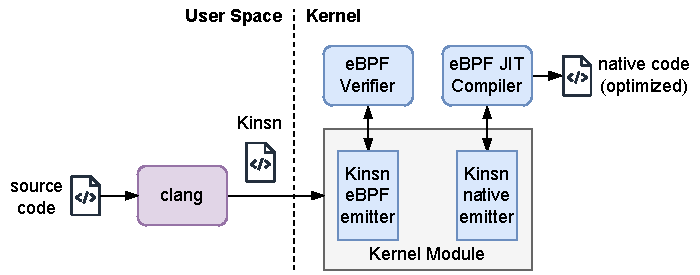
\includegraphics[width=\columnwidth]{figures/sec-4-pipeline.pdf}
\caption{The \lang compilation pipeline. The LLVM backend emits extended opcodes. A lowering stage expands each opcode into its proof sequence of vanilla eBPF, the eBPF verifier checks the lowered program, and a restore stage reinstates the extended opcodes. The eBPF JIT compiler then dispatches each extended opcode to its module-provided native emit callback.}
\label{fig:pipeline}
\end{figure}

Each \lang opcode is backed by a \emph{descriptor} that defines the opcode's semantics through a \emph{proof sequence}, a short fragment of ordinary eBPF instructions (C1). Before the main verification pass, a lowering stage walks the program and, for each \lang opcode, invokes the descriptor's \texttt{instantiate\_insn()} to expand the opcode into its proof sequence. The verifier then checks the lowered program with its existing transfer functions. After verification succeeds, a restore stage patches the original \lang opcodes back so that the program enters the JIT in its extended form. Proof sequences must satisfy structural constraints checked during lowering: no nested \lang opcodes, no function calls or exits, and no backward jumps, enforcing a single-entry, single-exit, straight-line property.

The descriptor also provides a \emph{native emit} callback for each supported architecture (C2). On encountering a \lang opcode, the eBPF JIT compiler calls the callback for the current architecture, which emits native instructions directly into the JIT image. The rotate descriptor, for example, emits a single \texttt{ROL} on x86-64 and a single \texttt{ROR} on ARM64. If no callback exists for the current architecture, the opcode falls back to its proof sequence, preserving correctness at the cost of the native performance benefit.

\lang instructions are packaged as kernel modules, with each descriptor living in its own module (C3). Adding a new instruction requires only writing such a module. No changes to the verifier, the JIT core, or the LLVM backend are needed. Table~\ref{tab:descriptors} lists the \todo{7} descriptors currently implemented.

\begin{table}[t]
\centering
\small
\caption{The \lang descriptors currently implemented, spanning five categories of hardware operations: bitwise rotation, conditional selection, bitfield extraction, endian-aware memory access, and speculation barriers. Every descriptor is supported on both x86-64 and ARM64.}
\label{tab:descriptors}
\begin{tabular*}{\columnwidth}{@{\extracolsep{\fill}}llll@{}}
\toprule
Descriptor & Proof sequence & x86-64 & ARM64 \\
\midrule
\texttt{rotate64} & 2 shifts + OR & \texttt{ROL} & \texttt{ROR} \\
\texttt{select64} & jump + 2 moves & \texttt{CMOV} & \texttt{CSEL} \\
\texttt{extract64} & shift + AND & \texttt{BEXTR} & \texttt{UBFX} \\
\texttt{endian\_load16} & load + bswap & \texttt{MOVBE} & \texttt{REV+LDRH} \\
\texttt{endian\_load32} & load + bswap & \texttt{MOVBE} & \texttt{REV+LDR} \\
\texttt{endian\_load64} & load + bswap & \texttt{MOVBE} & \texttt{REV+LDR} \\
\texttt{spec\_barrier} & identity (nop) & \texttt{LFENCE} & \texttt{DSB+ISB} \\
\bottomrule
\end{tabular*}
\end{table}


In the next section, we describe how we formally verify that the native emit is semantically consistent with the proof sequence the verifier checked.